% report, book, article, slides
%
% classe report para relatorios
% para essa aplicacao poderia ser qualquer uma
%
% para compilar
% $ pdflatex circulos.tex
% ou
% $ lualatex circulos.tex
% alo maria
\documentclass[a4paper]{report}
% usado para redimensionar as margens do papel
\usepackage{geometry}

% usado para introduzir os comandos de desenho
\usepackage{tikz}

% auto-explicativo
\geometry{left=1cm, right=1cm, top=1cm, bottom=1cm}

% usado para nao mostrar os numeros das paginas
\pagestyle{empty}
\begin{document}

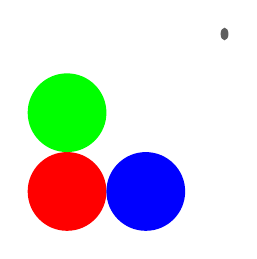
\begin{tikzpicture}
\fill[fill=red] (0,0) circle (0.5cm);
\fill[fill=blue] (1,0) circle (0.5cm);
\fill[fill=green] (0,1) circle (0.5cm);
\definecolor{cor}{rgb}{0.37,0.37,0.37}
\fill[color=cor] (2,2) ellipse(0.05cm and 0.08cm);
\end{tikzpicture}

\end{document}
